\documentclass[a4paper,12pt]{article}

\usepackage[cp1251]{inputenc}
\usepackage[T2A]{fontenc}
\usepackage[russian]{babel}
\usepackage{float}
\usepackage{subfigure}

\usepackage{booktabs}

\usepackage{graphicx}

\usepackage{amsthm}
\usepackage{import}

\usepackage{indentfirst}

\usepackage[labelsep=period,labelfont=bf,figurename={Рис.},figurewithin=none]{caption}

\usepackage{wrapfig}

\usepackage{amsmath}

\usepackage{amssymb}

\usepackage[a4paper,top=1.3cm,bottom=2cm,left=1.5cm,right=1.5cm,marginparwidth=0.75cm]{geometry}

\begin{document}

\begin{titlepage}
\begin{center}
    {\large МОСКОВСКИЙ ФИЗИКО-ТЕХНИЧЕСКИЙ ИНСТИТУТ (НАЦИОНАЛЬНЫЙ ИССЛЕДОВАТЕЛЬСКИЙ УНИВЕРСИТЕТ)}
\end{center}

\begin{center}
    {\large Физтех-школа радиотехники и компьютерных технологий}
\end{center}

\vspace{3.5cm}

\begin{center}
    
\includegraphics[width=0.4\linewidth]{hv_full.png}
\end{center}

\vspace{0.1cm}

{\huge
\begin{center}
    {\bf Лабораторная работа 2.3.1}\\
    Получение и измерение вакуума
\end{center}
}

\vspace{2cm}

\begin{flushright}
{\LARGE Автор:\\ Григорьев Даниил \\
\vspace{0.2cm}
Б01-407}
\end{flushright}

\vspace{3.5cm}
\begin{center}
    Долгопрудный 2025
\end{center}
\end{titlepage}

\section{Аннотация}
    \paragraph{Цель работы:} 1) измерение объемов форвакуумной и высоковакуумной
    частей установки;
    2) определение скорости откачки системы в стационарном режиме,
    а также по ухудшению и улучшению вакуума.
    \paragraph{В работе используются:} вакуумная установка с манометрами: масляным,
    термопарным и ионизационным.

\section{Теоретическая часть}
    \subsection{Процесс откачки}

    Пусть W --- объем газа, удаляемого из
    сосуда при данном давлении за единицу времени, $Q_i$ для различных значений
    $i$ обозначим различные притоки газа в сосуд (в единицах $PV$), такие как
    течи извне $Q_\text{и}$, десорбция с поверхностей внутри сосуда
    $Q_\text{д}$, обратный ток через насос $Q_\text{н}$. Тогда имеем:
    \begin{equation} -VdP = \left(PW - \sum Q_i\right)dt \end{equation} При
    достижении предельного вакуума устанавливается $P_{\text{пр}}$, и $dP = 0$.
    В таком случае: \begin{equation} W = \frac{\sum Q_i}{ P_{\text{пр}}}
    \end{equation} Поскольку обычно $Q_\text{и}$ постоянно, а $Q_\text{н}$ и
    $Q_\text{д}$ слабо зависят от времени, также считая постоянной W, можем
    проинтегрировать (1) и получить: \begin{equation} P - P_{\text{пр}} = (P_0 -
    P_{\text{пр}})\exp\left(-\frac{W}{V}t\right) \label{exp} \end{equation}
    Полная скорость откачки $W$, собственная скорость откачки насоса
    $W_{\text{н}}$ и проводимости элементов системы $C_1, C_2,\;\ldots$
    соотносятся согласно формуле (4), и это учтено в конструкции установки.
    \begin{equation} \frac{1}{W} = \frac{1}{W_\text{н}} + \frac{1}{C_1} +
    \frac{1}{C_2} + \ldots \end{equation}

\subsection{Течение газа через трубу}

	Характер течения газа существенно зависит от соотношения между размерами
	системы и длиной свободного пробега молекул. При атмосферном и форвакуумном
	давлениях  длина свободного пробега меньше диаметра трубок, и течение газа
	определяется его вязкостью, т.е. взаимодействием молекул. При переходе к
	высокому вакууму столкновения молекул между собой начинают играть меньшую
	роль, чем соударения со стенками.

	Для количества газа, протекающего через трубу длины $l$ и радиуса $r$ в
	условиях высокого вакуума, справедлива формула: \begin{equation}
	\frac{d(PV)}{dt} = \frac{4}{3}r^3\sqrt{\frac{2\pi RT}{\mu}}\cdot\frac{P_2 -
	P_1}{l} \label{kap} \end{equation} Если труба соединяет установку с
    насосом, то
	давлением $P_1$ у его конца можно пренебречь. Давление в сосуде $P = P_2$.
	Тогда пропускная способность трубы: \begin{equation} C_\text{тр} =
	\left(\frac{dV}{dt}\right)_\text{тр} = \frac{4r^3}{3l}\sqrt{\frac{2\pi
	RT}{\mu}} \label{ty} \end{equation}

\section{Экспериментальная установка}

    Установка изготовлена из стекла,
	и состоит из форвакуумного баллона (ФБ), высоковакуумного диффузионного
	насоса (ВН), высоковакуумного баллона (ВБ), масляного (М) и ионизационного
	(И) манометров, термопарных манометров ($\text{М}_1$ и $\text{М}_2$),
	форвакуумного насоса (ФН) и соединительных кранов ($\text{K}_1,
	\text{K}_2,\; \ldots \;\text{K}_6$) (Рис. 1). Кроме того, в
	состав установки входят: реостат и амперметр для регулирования тока
	нагревателя диффузионного насоса.

    \begin{figure}[H]
        \centering
        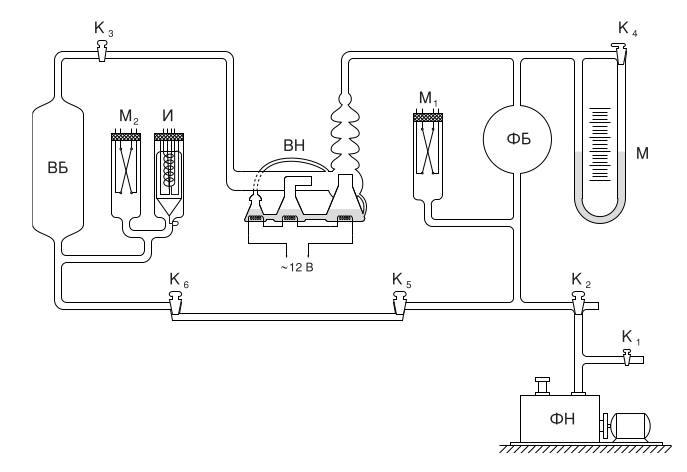
\includegraphics[scale=2]{stand.png}
        \caption{Схема экспериментальной установки}
        \label{facility}
    \end{figure}

\end{document}
